% The closed-disk model of the elliptic plane: projections and objects.
% Compile with:  pdflatex elliptic-disk-model.tex   (twice, for the references)
\documentclass[11pt,a4paper]{article}

\usepackage[T1]{fontenc}
\usepackage[utf8]{inputenc}
\usepackage{amsmath,amssymb,amsthm}
\usepackage[margin=2.6cm]{geometry}
\usepackage{tikz}
\usepackage{booktabs}
\usepackage{microtype}
\usepackage[colorlinks=true,linkcolor=black,citecolor=black,urlcolor=black]{hyperref}

\usetikzlibrary{arrows.meta,decorations.markings,positioning}

\newcommand{\RP}{\mathbb{R}\mathrm{P}}
\newcommand{\R}{\mathbb{R}}
\newcommand{\Sph}{\mathbb{S}^2}
\newcommand{\D}{\mathbb{D}}
\newcommand{\Hemi}{\mathbb{S}^{2}_{+}}
\newcommand{\proj}[1]{\pi_{\mathrm{#1}}}
\newcommand{\po}{\proj{o}}
\newcommand{\ps}{\proj{s}}
\newcommand{\nvec}{\mathbf{n}}
\newcommand{\vv}{\mathbf{v}}
\newcommand{\ee}{\mathbf{e}}
\newcommand{\uu}{\mathbf{u}}
\newcommand{\pp}{\mathbf{p}}
\newcommand{\qq}{\mathbf{q}}
\newcommand{\aaa}{\mathbf{a}}
\newcommand{\bb}{\mathbf{b}}
\newcommand{\cc}{\mathbf{c}}
\newcommand{\mm}{\mathbf{m}}
\newcommand{\tvec}{\mathbf{t}}
\newcommand{\zhat}{\hat{\mathbf{z}}}
\newcommand{\nuv}{\boldsymbol{\nu}}
\newcommand{\norm}[1]{\lVert #1 \rVert}
\newcommand{\abs}[1]{\lvert #1 \rvert}
\newcommand{\code}[1]{\texttt{#1}}

\theoremstyle{plain}
\newtheorem{proposition}{Proposition}[section]
\newtheorem{lemma}[proposition]{Lemma}
\newtheorem{corollary}[proposition]{Corollary}
\theoremstyle{definition}
\newtheorem{definition}[proposition]{Definition}
\theoremstyle{remark}
\newtheorem{remark}[proposition]{Remark}

\title{\bfseries The Closed-Disk Model of the Elliptic Plane\\[2mm]
       \large Projections and Constructed Objects}
\author{Aleksandar Ivanović}
\date{\today}

\begin{document}
\maketitle

\begin{abstract}
\noindent
This note collects the mathematics behind the interactive viewer in this
repository. It fixes the model --- the sphere with antipodal points identified,
drawn as a closed disk --- gives the two projections the viewer offers, and then
derives, for every object the program constructs, both its description on the
sphere and the curve it becomes on the page. The point of the derivations is
practical: knowing that the image of a line is a conic with a computable centre
and computable semi-axes is what lets the drawing and the \textsc{gclc} export
emit one exact arc instead of a few hundred short chords.
\end{abstract}

\tableofcontents

%======================================================================
\section{The model}

\subsection{The elliptic plane}

\begin{definition}
The \emph{elliptic plane} is the quotient
\[
  \RP^2 \;=\; \Sph/\{\pm 1\},
  \qquad
  \Sph=\{\vv\in\R^3 : \norm{\vv}=1\},
\]
in which a point is an antipodal pair $[\vv]=\{\vv,-\vv\}$, and a \emph{line} is
the image of a great circle. The metric is inherited from the round sphere.
\end{definition}

Two facts govern everything that follows. First, two distinct points lie on
exactly one line and two distinct lines meet in exactly one point: \emph{there
are no parallels}, and point and line play symmetric roles. Second, because the
identification halves the sphere, every distance is at most $\pi/2$ and the
total area is $2\pi$ rather than $4\pi$.

\subsection{Representatives and the closed disk}

Each class $[\vv]$ has a representative on the closed upper hemisphere
\[
  \Hemi=\{\vv\in\Sph : v_3\ge 0\},
\]
unique except on the equator $v_3=0$, where $\vv$ and $-\vv$ both lie in
$\Hemi$ and are the same elliptic point. Write
\begin{equation}
  \label{eq:upper}
  \operatorname{up}(\vv)=
  \begin{cases}
    -\vv, & v_3<0,\\
    \phantom{-}\vv, & v_3\ge 0,
  \end{cases}
\end{equation}
for the choice of that representative.

\begin{remark}[why the code compares against $-\varepsilon$ and not $0$]
In the program \eqref{eq:upper} flips only when $v_3<-\varepsilon$. On the
equator the two representatives are equally correct, and a sampled curve whose
endpoint lands at $v_3=-10^{-17}$ must not be thrown to the other side of the
disk; the tolerance keeps a curve that ends on the rim in one piece.
\end{remark}

A \emph{projection} is a homeomorphism $\pi\colon\Hemi\to\overline{\D}$ onto the
closed unit disk $\overline{\D}=\{\uu\in\R^2:\norm{\uu}\le 1\}$. The picture is
then the disk with \emph{diametrically opposite boundary points identified},
\[
  \uu \sim -\uu \qquad (\norm{\uu}=1),
\]
which is the residue of the antipodal identification and the reason the rim is
drawn dashed. Both projections below fix the rim pointwise, so this
identification --- and therefore the model, the picking and every measurement
--- is the same in either view.

%======================================================================
\section{The projections}
\label{sec:projections}

\subsection{Orthogonal projection}

\begin{definition}
\emph{Orthogonal} (vertical, ``seen straight down'') projection is
\begin{equation}
  \label{eq:ortho}
  \po(\vv)=(v_1,v_2),
  \qquad
  \po^{-1}(x,y)=\bigl(x,\;y,\;\sqrt{1-x^2-y^2}\bigr).
\end{equation}
\end{definition}

It is a bijection $\Hemi\to\overline{\D}$ and fixes the rim. It is neither
conformal nor area-preserving; it compresses radially near the boundary, which
is why a right angle drawn far from the centre visibly leans.

\subsection{Stereographic projection}

\begin{definition}
\emph{Stereographic} projection from the south pole $S=(0,0,-1)$ is
\begin{equation}
  \label{eq:stereo}
  \ps(\vv)=\frac{(v_1,v_2)}{1+v_3},
  \qquad
  \ps^{-1}(x,y)=\frac{\bigl(2x,\;2y,\;1-x^2-y^2\bigr)}{1+x^2+y^2}.
\end{equation}
\end{definition}

\begin{lemma}
$\ps$ maps $\Hemi$ bijectively onto $\overline{\D}$ and fixes the rim
pointwise.
\end{lemma}

\begin{proof}
For $\vv\in\Sph$ with $\norm{\ps(\vv)}^2=(1-v_3^2)/(1+v_3)^2=(1-v_3)/(1+v_3)$,
which is a decreasing function of $v_3$ equal to $1$ at $v_3=0$ and to $0$ at
$v_3=1$. Hence $v_3\ge0 \iff \norm{\ps(\vv)}\le1$, and $v_3=0$ gives
$\ps(\vv)=(v_1,v_2)$, the identity on the equator. Formula \eqref{eq:stereo} for
$\ps^{-1}$ is verified by substitution.
\end{proof}

\begin{remark}
The inverse in \eqref{eq:stereo} is a \emph{rational} map, whereas
$\po^{-1}$ involves $\sqrt{1-x^2-y^2}$, whose derivative blows up at the rim.
This is a real numerical difference; see \S\ref{sec:numerics}.
\end{remark}

\begin{figure}[t]
\centering
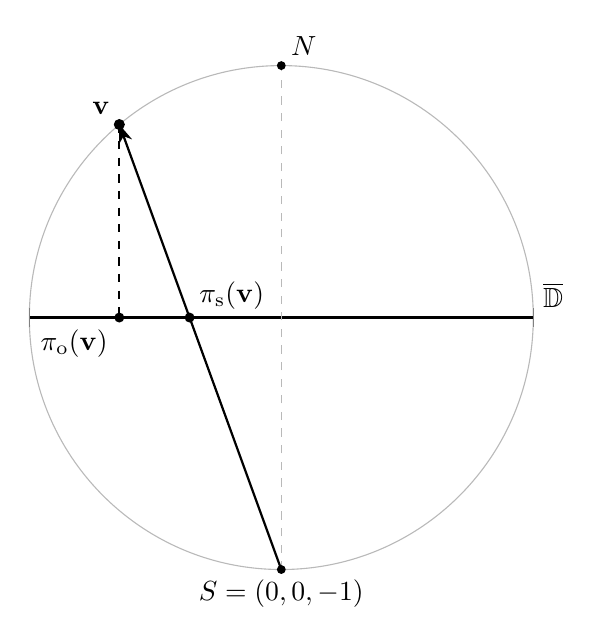
\begin{tikzpicture}[scale=1.0,>=Stealth]
  \def\Rad{3.2}
  \pgfmathsetmacro{\ang}{130}
  \pgfmathsetmacro{\px}{\Rad*cos(\ang)}
  \pgfmathsetmacro{\pz}{\Rad*sin(\ang)}
  \pgfmathsetmacro{\ox}{\px}
  \pgfmathsetmacro{\sx}{\Rad*cos(\ang)/(1+sin(\ang))}

  % sphere cross-section
  \draw[gray!55] (0,0) circle (\Rad);
  \draw[very thick] (-\Rad,0) -- (\Rad,0);
  \draw[gray!55,dashed] (0,-\Rad) -- (0,\Rad);

  \fill (0,-\Rad) circle (1.6pt) node[below] {$S=(0,0,-1)$};
  \fill (0,\Rad) circle (1.6pt) node[above right] {$N$};

  % the point
  \fill (\px,\pz) circle (2pt) node[above left] {$\vv$};

  % orthogonal ray
  \draw[thick,dashed] (\px,\pz) -- (\ox,0);
  \fill (\ox,0) circle (1.8pt);
  \node[below left=1pt] at (\ox,0) {$\po(\vv)$};

  % stereographic ray
  \draw[thick,->] (0,-\Rad) -- (\px,\pz);
  \fill (\sx,0) circle (1.8pt);
  \node[above right=1pt and 0pt] at (\sx,-0.05) {$\ps(\vv)$};

  \node[right] at (\Rad,0.28) {$\overline{\D}$};
  \draw[gray] (\Rad,-0.12) -- (\Rad,0.12);
  \draw[gray] (-\Rad,-0.12) -- (-\Rad,0.12);
\end{tikzpicture}
\caption{The two projections in a vertical cross-section. Orthogonal projection
drops the point straight down; stereographic projection follows the ray from the
south pole. Both send the closed upper hemisphere onto the closed unit disk and
both fix the rim.}
\label{fig:cross-section}
\end{figure}

\subsection{The metric each one induces}

Pulling the round metric of $\Sph$ back through $\pi^{-1}$ turns the disk into a
metric object; the two answers are quite different and explain what each view is
good for.

\begin{proposition}[orthogonal]
With $r^2=x^2+y^2$ and $(x,y)$ polar as $x=r\cos\theta$, $y=r\sin\theta$,
\begin{equation}
  ds_{\mathrm{o}}^2
    =dx^2+dy^2+\frac{(x\,dx+y\,dy)^2}{1-x^2-y^2}
    =\frac{dr^2}{1-r^2}+r^2\,d\theta^2,
  \qquad
  dA_{\mathrm{o}}=\frac{dx\,dy}{\sqrt{1-x^2-y^2}}.
\end{equation}
Substituting $r=\sin\rho$ gives $ds_{\mathrm{o}}^2=d\rho^2+\sin^2\!\rho\;d\theta^2$:
the radial coordinate $r$ is the \emph{sine} of the true distance $\rho$ from
the centre, and the rim $r=1$ is at distance exactly $\pi/2$.
\end{proposition}

\begin{proof}
Differentiate $z=\sqrt{1-x^2-y^2}$ to get $dz=-(x\,dx+y\,dy)/z$ and substitute
into $ds^2=dx^2+dy^2+dz^2$. In polar coordinates $x\,dx+y\,dy=r\,dr$, so the
extra term is $r^2dr^2/(1-r^2)$ and $dr^2+r^2dr^2/(1-r^2)=dr^2/(1-r^2)$.
\end{proof}

\begin{proposition}[stereographic]
\begin{equation}
  ds_{\mathrm{s}}^2=\frac{4\,(dx^2+dy^2)}{(1+x^2+y^2)^2},
  \qquad
  dA_{\mathrm{s}}=\frac{4\,dx\,dy}{(1+x^2+y^2)^2}.
\end{equation}
The metric is a positive multiple of the Euclidean one, so $\ps$ is
\emph{conformal}: an angle measured on the page is the angle of the geometry,
everywhere and exactly.
\end{proposition}

That single line is the whole trade-off. In the orthogonal view distances read
off the page by a fixed rule ($\rho=\arcsin r$ from the centre) but angles are
distorted; in the conformal view angles are honest but distance is not read off
the page at all.

%======================================================================
\section{Points}

\begin{definition}
A \emph{point} of the construction is an elliptic point $[\vv]$, stored by its
representative $\vv\in\Hemi$, $\norm{\vv}=1$.
\end{definition}

A click at $(x,y)$ becomes $\vv=\pi^{-1}(x,y)$ for whichever projection $\pi$ is
in force, after clamping outside points onto the rim:
\begin{equation}
  \operatorname{clamp}(x,y)=
  \begin{cases}
    (x,y)/r, & r>1,\\
    (x,y), & r\le1,
  \end{cases}
  \qquad r=\sqrt{x^2+y^2}.
\end{equation}

Points are of two kinds. A \emph{free} point carries its own position and can be
dragged. A \emph{derived} point carries a rule --- a meet (\S\ref{sec:meet}) or a
pole (\S\ref{sec:duality}) --- and recomputes its vector from its parents each
time it is asked, which is what makes the whole figure move when one vertex is
dragged.

%======================================================================
\section{Lines}
\label{sec:lines}

\begin{definition}
The \emph{line} through two distinct points $[\pp],[\qq]$ is the great circle
\[
  \ell_\nvec=\{\vv\in\Sph : \nvec\cdot\vv=0\},
  \qquad
  \nvec=\frac{\pp\times\qq}{\norm{\pp\times\qq}} ,
\]
and $\nvec$ is defined up to sign, i.e.\ it is itself an elliptic point. The
cross product vanishes exactly when $[\pp]=[\qq]$, in which case infinitely many
lines pass through them and the construction refuses.
\end{definition}

Writing $\nuv=(n_1,n_2)$ and $\hat\nuv=\nuv/\norm{\nuv}$, so that
$\norm{\nuv}^2=1-n_3^2$, we can say exactly what a line looks like on the page.

\subsection{Orthogonal image: half an ellipse}

\begin{proposition}
\label{prop:line-ellipse}
Let $\abs{n_3}<1$ and $\norm{\nuv}>0$. Then $\po(\ell_\nvec)$ is half of the
ellipse centred at the origin with
\[
  \text{semi-major axis } 1 \text{ along } \hat\nuv^{\perp}=\frac{(-n_2,n_1)}{\norm{\nuv}},
  \qquad
  \text{semi-minor axis } \abs{n_3} \text{ along } \hat\nuv .
\]
The half drawn is the one containing $-\operatorname{sgn}(n_3)\,\abs{n_3}\hat\nuv$,
and it joins the antipodal rim points $\pm\hat\nuv^{\perp}$.
\end{proposition}

\begin{proof}
A point of the disk is on the image iff
$n_1x+n_2y+n_3\sqrt{1-x^2-y^2}=0$. Squaring,
\[
  n_3^2\,(1-x^2-y^2)=(n_1x+n_2y)^2
  \;\Longleftrightarrow\;
  \uu^{\!\top}\!\bigl(\nuv\nuv^{\!\top}+n_3^2 I\bigr)\uu=n_3^2,
  \qquad \uu=(x,y)^{\!\top}.
\]
The matrix $M=\nuv\nuv^{\!\top}+n_3^2I$ has eigenvector $\hat\nuv$ with
eigenvalue $\norm{\nuv}^2+n_3^2=1$ and eigenvector $\hat\nuv^{\perp}$ with
eigenvalue $n_3^2$. In those coordinates, $\uu=s\,\hat\nuv+t\,\hat\nuv^{\perp}$,
the equation reads $s^2+n_3^2t^2=n_3^2$, i.e.
\[
  \frac{s^2}{n_3^2}+\frac{t^2}{1}=1 .
\]
So the semi-axis along $\hat\nuv$ is $\abs{n_3}\le1$ and the one along
$\hat\nuv^{\perp}$ is $1$. Squaring doubled the solution set: only the half with
$n_1x+n_2y$ and $n_3$ of opposite sign survives, and that half is bounded by
$t=\pm1$, $s=0$, the two rim points $\pm\hat\nuv^{\perp}$. Finally, the point of
$\ell_\nvec$ of greatest height is
$(\zhat-n_3\nvec)/\norm{\zhat-n_3\nvec}$, whose horizontal part is
$-n_3\nuv/\norm{\nuv}$; this is the apex of the drawn half.
\end{proof}

\begin{corollary}[degenerate cases]
$n_3=0$: the ellipse collapses onto its major axis and the line is drawn as the
\emph{diameter} along $\hat\nuv^{\perp}$. $\abs{n_3}=1$ (the equator): the line
is the \emph{whole rim circle}. These are exactly the two cases in which the
program returns no conic and draws something else.
\end{corollary}

\subsection{Stereographic image: a circular arc}

\begin{proposition}
\label{prop:line-circle}
Let $n_3\neq0$. Then $\ps(\ell_\nvec)$ is the arc, inside $\overline{\D}$, of the
circle
\begin{equation}
  \label{eq:line-circle}
  \norm{\uu-\cc}=\varrho,
  \qquad
  \cc=\frac{(n_1,n_2)}{n_3},
  \qquad
  \varrho=\frac{1}{\abs{n_3}} .
\end{equation}
If $n_3=0$ the image is the diameter along $\hat\nuv^{\perp}$, as before.
\end{proposition}

\begin{proof}
Substitute \eqref{eq:stereo} into $\nvec\cdot\vv=0$. With $q=x^2+y^2$,
\[
  \frac{2n_1x+2n_2y+n_3(1-q)}{1+q}=0
  \;\Longleftrightarrow\;
  n_3\,q-2n_1x-2n_2y-n_3=0 .
\]
For $n_3\neq0$ divide by $n_3$ and complete the square:
$\norm{\uu-\cc}^2=1+\norm{\cc}^2=(n_3^2+n_1^2+n_2^2)/n_3^2=1/n_3^2$.
For $n_3=0$ the equation is linear, $n_1x+n_2y=0$.
\end{proof}

\begin{corollary}[the identification is visible]
\label{cor:orthogonal-circle}
The circle \eqref{eq:line-circle} meets the unit circle where $\cc\cdot\uu=0$,
i.e.\ at the two \emph{antipodal} rim points $\pm\hat\cc^{\perp}=\pm\hat\nuv^{\perp}$
--- the same pair as in Proposition~\ref{prop:line-ellipse}.
\end{corollary}

\begin{proof}
Subtract $\norm{\uu}^2=1$ from $\norm{\uu-\cc}^2=1+\norm{\cc}^2$ to get
$-2\cc\cdot\uu=0$.
\end{proof}

\begin{figure}[t]
\centering
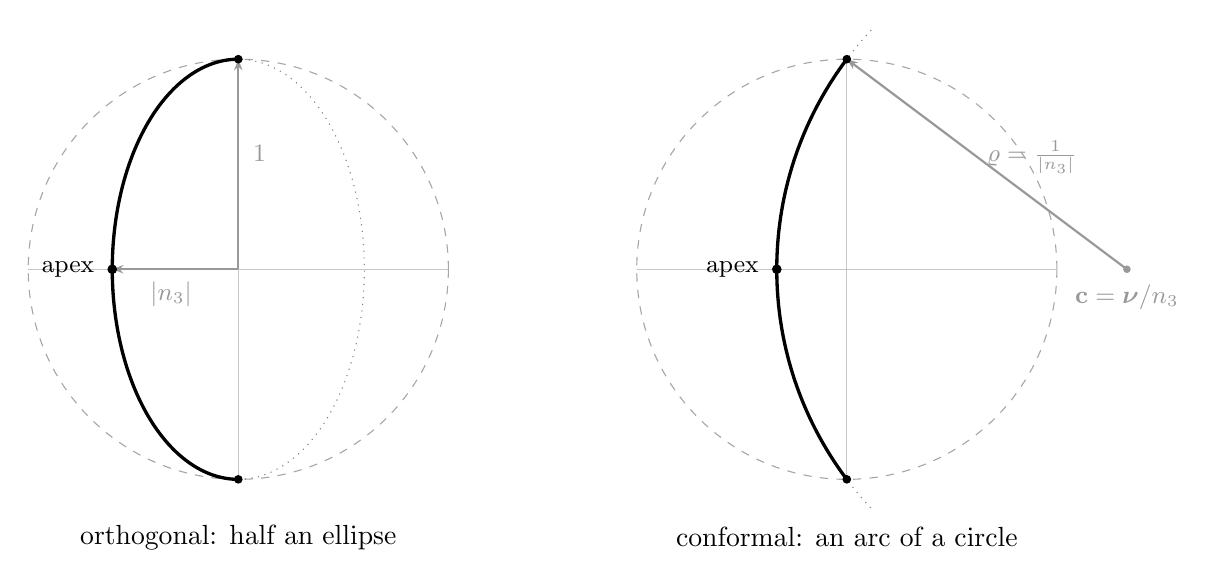
\begin{tikzpicture}[scale=0.92]
  \def\Rad{2.9}
  % --- orthogonal ---
  \begin{scope}
    \draw[dashed,gray!70] (0,0) circle (\Rad);
    \draw[gray!45] (-\Rad,0) -- (\Rad,0);
    \draw[gray!45] (0,-\Rad) -- (0,\Rad);
    % n = (0.8, 0, 0.6): semi-minor 0.6 along x, semi-major 1 along y,
    % the drawn half is x <= 0
    \draw[thin,gray,dotted,domain=-90:90,samples=160,smooth,variable=\t]
      plot ({0.6*\Rad*cos(\t)},{\Rad*sin(\t)});
    \draw[very thick,domain=90:270,samples=200,smooth,variable=\t]
      plot ({0.6*\Rad*cos(\t)},{\Rad*sin(\t)});
    % the two semi-axes
    \draw[-{Stealth[length=4pt]},thick,gray!80] (0,0) -- (0,\Rad);
    \draw[-{Stealth[length=4pt]},thick,gray!80] (0,0) -- (-0.6*\Rad,0);
    \node[gray!80,right=1pt] at (0.03,{0.55*\Rad}) {\small $1$};
    \node[gray!80,below] at (-0.32*\Rad,-0.04) {\small $\abs{n_3}$};
    \fill (0,\Rad) circle (1.7pt);
    \fill (0,-\Rad) circle (1.7pt);
    \fill (-0.6*\Rad,0) circle (1.9pt);
    \node[left=3pt] at (-0.6*\Rad,0) {\small apex};
    \node at (0,-\Rad-0.8) {orthogonal: half an ellipse};
  \end{scope}
  % --- stereographic ---
  \begin{scope}[xshift=8.4cm]
    \draw[dashed,gray!70] (0,0) circle (\Rad);
    \draw[gray!45] (-\Rad,0) -- (\Rad,0);
    \draw[gray!45] (0,-\Rad) -- (0,\Rad);
    % same n: centre (4/3, 0)*R, radius (5/3)*R
    \begin{scope}
      \clip (-1.15*\Rad,-1.15*\Rad) rectangle (1.55*\Rad,1.15*\Rad);
      \draw[thin,gray,dotted] ({1.3333*\Rad},0) circle ({1.6667*\Rad});
    \end{scope}
    \begin{scope}
      \clip (0,0) circle (\Rad);
      \draw[very thick] ({1.3333*\Rad},0) circle ({1.6667*\Rad});
    \end{scope}
    % centre and radius
    \draw[-{Stealth[length=4pt]},thick,gray!80] ({1.3333*\Rad},0) -- (0,\Rad);
    \node[gray!80,above right=-1pt and 0pt] at ({0.62*\Rad},{0.42*\Rad})
      {\small $\varrho=\tfrac{1}{\abs{n_3}}$};
    \fill[gray!80] ({1.3333*\Rad},0) circle (1.5pt);
    \node[gray!80,below] at ({1.3333*\Rad},-0.08) {\small $\cc=\nuv/n_3$};
    \fill (0,\Rad) circle (1.7pt);
    \fill (0,-\Rad) circle (1.7pt);
    \fill (-0.3333*\Rad,0) circle (1.9pt);
    \node[left=3pt] at (-0.3333*\Rad,0) {\small apex};
    \node at (0,-\Rad-0.8) {conformal: an arc of a circle};
  \end{scope}
\end{tikzpicture}
\caption{One and the same elliptic line, $\nvec=(0.8,\,0,\,0.6)$, drawn both
ways. Both curves run between the same pair of antipodal rim points
$\pm\hat\nuv^{\perp}=(0,\pm1)$ (Corollary~\ref{cor:orthogonal-circle}), and the
two marked apexes are the images of the same point $(-0.6,0,0.8)$ of the sphere.
The dotted continuation on the left is the half of the ellipse that the lower
hemisphere would project to; it is \emph{not} part of the line.}
\label{fig:two-views}
\end{figure}

\subsection{Parametrisation, and which half is drawn}

For sampling and for cutting segments the program uses a parametrisation rather
than the implicit equations. Choose an orthonormal basis $\ee_1,\ee_2$ of
$\nvec^{\perp}$ and set
\begin{equation}
  \label{eq:arc-param}
  \gamma(t)=\cos t\;\ee_1+\sin t\;\ee_2 .
\end{equation}
Its height is
\begin{equation}
  \label{eq:height}
  \gamma_3(t)=e_{1,3}\cos t+e_{2,3}\sin t=R\cos(t-\varphi),
  \qquad
  \varphi=\operatorname{atan2}(e_{2,3},e_{1,3}),\quad R=\sqrt{1-n_3^2},
\end{equation}
so $\gamma_3\ge0$ precisely on the half-turn
\begin{equation}
  \label{eq:line-range}
  t\in[\varphi-\tfrac{\pi}{2},\;\varphi+\tfrac{\pi}{2}] .
\end{equation}
That interval \emph{is} the line: a half-turn, mapping onto half the ellipse (or
onto the circular arc). The equator, $R=0$, is the exception and takes the full
turn $[0,2\pi]$.

%======================================================================
\section{Distance and segments}

\begin{definition}
The \emph{distance} between two elliptic points is the angle between their
representatives, folded by the identification:
\begin{equation}
  \label{eq:distance}
  d([\pp],[\qq])=\arccos\bigl(\abs{\pp\cdot\qq}\bigr)\in[0,\tfrac{\pi}{2}].
\end{equation}
\end{definition}

The absolute value is the whole content of the identification: whichever of
$\pm\qq$ is nearer to $\pp$ is the one that counts, and no two points are ever
more than a quarter turn apart. The rim is at distance exactly $\pi/2$ from the
centre.

\subsection{The shortest segment, and why it can arrive in two pieces}

Let $\pp,\qq$ lie on $\ell_\nvec$ with parameters $t_p,t_q$ in
\eqref{eq:arc-param}. Reduce
\begin{equation}
  \delta \equiv (t_q-t_p+\pi)\bmod 2\pi-\pi\in(-\pi,\pi],
  \qquad
  \delta \leftarrow \delta-\operatorname{sgn}(\delta)\,\pi
  \quad\text{if } \abs{\delta}>\tfrac{\pi}{2},
\end{equation}
the second step choosing the antipodal representative of $\qq$ when it is the
nearer one. The segment is then $\gamma$ on $[t_p,\,t_p+\delta]$, of length
$\abs{\delta}=d(\pp,\qq)$.

This arc need not stay in the upper hemisphere. By \eqref{eq:height} the height
vanishes at $t=\varphi\pm\pi/2$; since $\abs{\delta}\le\pi/2$ the arc crosses at
most one of those, at a parameter $t_\ast$ strictly between its ends. Splitting
there and applying $\operatorname{up}$ to each piece --- which on an arc means
replacing $(\ee_1,\ee_2)$ by $(-\ee_1,-\ee_2)$ --- gives \emph{one or two} drawn
arcs. Geometrically: the shortest route leaves the disk through the rim and
re-enters at the diametrically opposite boundary point.

\begin{remark}
The cut is computed from \eqref{eq:height} analytically, not detected from the
samples, so the two pieces do not depend on how finely the curve is drawn ---
and the export can emit them as two exact arcs.
\end{remark}

%======================================================================
\section{Duality: pole and polar}
\label{sec:duality}

\begin{definition}
The \emph{polar} of a point $[\pp]$ is the line $\ell_{\pp}$ with normal $\pp$;
the \emph{pole} of a line $\ell_\nvec$ is the point $[\nvec]$.
\end{definition}

\begin{proposition}
$\ell_\pp=\{[\vv] : d([\pp],[\vv])=\pi/2\}$, and pole and polar are mutually
inverse: the pole of the polar of $[\pp]$ is $[\pp]$.
\end{proposition}

\begin{proof}
$d([\pp],[\vv])=\pi/2\iff\abs{\pp\cdot\vv}=0\iff\vv\in\ell_\pp$. The second claim
is immediate from the definitions, both sides being the class $[\pp]$.
\end{proof}

So a point and a line are the same kind of object; the viewer offers them as one
tool. Dualising a whole figure exchanges ``lies on'' with ``passes through'',
collinear points with concurrent lines.

\subsection{Meet}
\label{sec:meet}

\begin{proposition}
Two distinct lines $\ell_{\nvec_1},\ell_{\nvec_2}$ meet in exactly one point,
\begin{equation}
  \label{eq:meet}
  [\nvec_1\times\nvec_2].
\end{equation}
\end{proposition}

\begin{proof}
$\vv$ lies on both iff it is orthogonal to $\nvec_1$ and $\nvec_2$, i.e.\ spans
$(\operatorname{span}\{\nvec_1,\nvec_2\})^{\perp}$, a line of $\R^3$ when
$\nvec_1\neq\pm\nvec_2$; its two unit vectors are one elliptic point.
\end{proof}

This is exactly dual to $\nvec=\pp\times\qq$ for the join, and it is why the
elliptic plane has no parallels.

\subsection{Perpendiculars}

\begin{proposition}
\label{prop:perp}
Let $[\pp]$ be a point and $\ell_\nvec$ a line with $[\pp]\neq[\nvec]$. There is
exactly one line through $[\pp]$ perpendicular to $\ell_\nvec$, namely
\begin{equation}
  \label{eq:perp}
  \ell_\mm,\qquad \mm=\frac{\pp\times\nvec}{\norm{\pp\times\nvec}},
\end{equation}
which is the join of $[\pp]$ and the pole $[\nvec]$. Its foot --- the point of
$\ell_\nvec$ nearest $[\pp]$ --- is
\begin{equation}
  \label{eq:foot}
  [\,\nvec\times\mm\,],
\end{equation}
and
\begin{equation}
  \label{eq:dist-to-line}
  d\bigl([\pp],\ell_\nvec\bigr)=\arcsin\bigl(\abs{\pp\cdot\nvec}\bigr)
  =\tfrac{\pi}{2}-d\bigl([\pp],[\nvec]\bigr).
\end{equation}
If $[\pp]=[\nvec]$ --- the point \emph{is} the pole --- then every line through
$[\pp]$ is perpendicular to $\ell_\nvec$ and \eqref{eq:perp} degenerates.
\end{proposition}

\begin{proof}
Two lines are perpendicular iff their normals are orthogonal,
$\nvec\cdot\mm=0$; and $\ell_\mm$ passes through $[\pp]$ iff
$\pp\cdot\mm=0$. Both hold for $\mm\propto\pp\times\nvec$, and that vector is
determined up to sign whenever $\pp\times\nvec\neq0$. Since $\mm\perp\nvec$, the
pole $[\nvec]$ lies on $\ell_\mm$: every line through the pole of $\ell_\nvec$
crosses it at a right angle. Equation~\eqref{eq:foot} is \eqref{eq:meet} applied
to $\ell_\nvec$ and $\ell_\mm$. For \eqref{eq:dist-to-line}, decompose
$\pp=(\pp\cdot\nvec)\nvec+\pp^{\parallel}$ with $\pp^{\parallel}\in\nvec^{\perp}$;
the nearest point of $\ell_\nvec$ is $[\pp^{\parallel}]$ and
$\cos d=\norm{\pp^{\parallel}}=\sqrt{1-(\pp\cdot\nvec)^2}$.
\end{proof}

\begin{corollary}
All perpendiculars to a given line are concurrent --- they meet at its pole.
Dropping perpendiculars from two different points onto one line and watching
them cross at the pole is the cleanest check that the construction is right.
\end{corollary}

%======================================================================
\section{Angles, triangles and area}

\subsection{Tangents and the angle at a vertex}

For $[\aaa]\neq[\bb]$ let $\bb^{\ast}=\operatorname{sgn}(\aaa\cdot\bb)\,\bb$ be
the nearer representative. The unit tangent at $\aaa$ along the shortest arc
towards $[\bb]$ is
\begin{equation}
  \label{eq:tangent}
  \tvec(\aaa,\bb)=\frac{\bb^{\ast}-(\aaa\cdot\bb^{\ast})\aaa}
                       {\norm{\bb^{\ast}-(\aaa\cdot\bb^{\ast})\aaa}},
\end{equation}
and the angle at $[\aaa]$ in the ``triangle'' $\aaa\bb\cc$ is
\begin{equation}
  \label{eq:angle}
  \alpha=\arccos\bigl(\tvec(\aaa,\bb)\cdot\tvec(\aaa,\cc)\bigr)\in[0,\pi].
\end{equation}
At exactly $d=\pi/2$ both representatives of $\bb$ are equally near and the
direction is defined only up to sign.

\subsection{Girard's theorem}

\begin{proposition}[Girard]
A triangle whose three shortest sides bound a disk has area
\begin{equation}
  \label{eq:girard}
  \operatorname{Area}=\alpha+\beta+\gamma-\pi .
\end{equation}
\end{proposition}

The excess is therefore not an error term but the area itself. It is positive
for every genuine triangle --- the angle sum always beats $\pi$ --- and it goes
to $0$ as the triangle shrinks, which is Euclidean geometry appearing in the
limit.

\subsection{When three points bound nothing}

Not every triple bounds a triangle, and \eqref{eq:girard} must not be applied
blindly.

\begin{proposition}
\label{prop:bounds}
Walk the three shortest sides $[\aaa]\to[\bb]\to[\cc]\to[\aaa]$, at each step
lifting to the nearer representative of the far endpoint. The walk returns to
$+\aaa$ if and only if
\begin{equation}
  \label{eq:bounds}
  (\aaa\cdot\bb)(\bb\cdot\cc)(\cc\cdot\aaa)\;>\;0 ,
\end{equation}
and to $-\aaa$ otherwise.
\end{proposition}

\begin{proof}
Set $\bb_1=\sigma_1\bb$ with $\sigma_1=\operatorname{sgn}(\aaa\cdot\bb)$. Then
$\cc_1=\operatorname{sgn}(\bb_1\cdot\cc)\,\cc=\sigma_1\operatorname{sgn}(\bb\cdot\cc)\,\cc$,
and finally
$\aaa_1=\operatorname{sgn}(\cc_1\cdot\aaa)\,\aaa
      =\operatorname{sgn}(\aaa\cdot\bb)\operatorname{sgn}(\bb\cdot\cc)\operatorname{sgn}(\cc\cdot\aaa)\,\aaa$,
because the leading $\sigma_1$ appears twice and squares away.
\end{proof}

When the product is negative the closed curve made of the three sides runs out
through the rim and back in on the other side; it is a non-contractible loop in
$\RP^2$, it bounds no disk, and Girard's formula has nothing to apply to. The
program reports that rather than printing a number, and pulling one vertex back
in restores the area.

\subsection{The marks that are drawn}

Both angle marks are constructed \emph{on the sphere} and then projected, so
they are honest about the distortion of the view rather than faking a square
corner.

\paragraph{Angle arc.} With $\tvec_1=\tvec(\aaa,\bb)$, $\tvec_2=\tvec(\aaa,\cc)$,
$\theta$ the angle \eqref{eq:angle} and
$\tvec_{\perp}=\dfrac{\tvec_2-(\tvec_1\cdot\tvec_2)\tvec_1}
                     {\norm{\tvec_2-(\tvec_1\cdot\tvec_2)\tvec_1}}$,
the mark at radius $\rho$ (the program uses $\rho=0.13$) is
\begin{equation}
  s\;\longmapsto\;\cos\rho\;\aaa+\sin\rho\,\bigl(\cos s\;\tvec_1+\sin s\;\tvec_{\perp}\bigr),
  \qquad s\in[0,\theta].
\end{equation}

\paragraph{Right-angle mark.} At a foot $\mathbf{f}$ where $\ell_{\nvec_1}$ and
$\ell_{\nvec_2}$ cross, the two unit tangents along the lines are
$\tvec_i=\widehat{\nvec_i\times\mathbf{f}}$, and the corners
\begin{equation}
  \widehat{\mathbf{f}+h\tvec_1},\qquad
  \widehat{\mathbf{f}+h(\tvec_1+\tvec_2)},\qquad
  \widehat{\mathbf{f}+h\tvec_2}
\end{equation}
(with $\widehat{\;\cdot\;}$ meaning normalise, then fold up by
\eqref{eq:upper}) form a small square on the sphere. Under $\po$ it comes out as
a slanted parallelogram except near the centre; under $\ps$ it squares up by
itself, because $\ps$ is conformal. Both marks are dropped altogether when they
would straddle the rim, where they would tear across the disk.

%======================================================================
\section{Circles}

\begin{definition}
The \emph{circle} of centre $[\aaa]$ and radius $r\in(0,\pi/2]$ is
$\{[\vv]:d([\aaa],[\vv])=r\}$, i.e.\ the plane section
$\aaa\cdot\vv=\cos r$ of the sphere, of Euclidean centre $\cos r\,\aaa$ and
Euclidean radius $\sin r$.
\end{definition}

At $r=\pi/2$ it degenerates to the polar line of its centre --- in this geometry
a circle of large enough radius \emph{is} a line, which is the cleanest way to
see the duality at work.

\begin{proposition}[orthogonal image]
\label{prop:circle-ortho}
Let $\ee_1,\ee_2$ be an orthonormal basis of $\aaa^{\perp}$ and let
$A=\sin r\,[\,\ee_1^{\,xy}\;\;\ee_2^{\,xy}\,]\in\R^{2\times2}$ be the matrix of
their horizontal parts. Then $\po$ of the circle is the ellipse
\begin{equation}
  \uu(t)=\cos r\,\aaa^{xy}+A\binom{\cos t}{\sin t},
\end{equation}
centred at $\cos r\,\aaa^{xy}$, whose semi-axes are the singular values of $A$
taken along its left singular vectors. If $A=U\Sigma V^{\!\top}$, the semi-axis
vectors are $\sigma_1\uu_1$ and $\sigma_2\uu_2$.
\end{proposition}

\begin{proof}
Parametrise the plane section as
$\vv(t)=\cos r\,\aaa+\sin r\,(\cos t\,\ee_1+\sin t\,\ee_2)$ and drop the third
coordinate. The image of the unit circle under a linear map $A$ is an ellipse
whose principal axes are given by the singular value decomposition.
\end{proof}

\begin{proposition}[stereographic image]
If $a_3+\cos r\neq0$, then $\ps$ of the circle is the circle
\begin{equation}
  \label{eq:circle-stereo}
  \norm{\uu-\cc}=\varrho,
  \qquad
  \cc=\frac{(a_1,a_2)}{a_3+\cos r},
  \qquad
  \varrho=\frac{\sin r}{\abs{a_3+\cos r}} .
\end{equation}
If $a_3+\cos r=0$ the circle passes through the south pole and its image is a
straight line.
\end{proposition}

\begin{proof}
Substitute \eqref{eq:stereo} into $\aaa\cdot\vv=\cos r$. With $q=x^2+y^2$ and
$c=\cos r$,
\[
  2a_1x+2a_2y+a_3(1-q)=c\,(1+q)
  \;\Longleftrightarrow\;
  (a_3+c)\,q-2a_1x-2a_2y-(a_3-c)=0 .
\]
Dividing by $a_3+c$ and completing the square gives centre
$(a_1,a_2)/(a_3+c)$ and
\[
  \varrho^2=\frac{a_1^2+a_2^2}{(a_3+c)^2}+\frac{a_3-c}{a_3+c}
          =\frac{a_1^2+a_2^2+a_3^2-c^2}{(a_3+c)^2}
          =\frac{1-c^2}{(a_3+c)^2}=\frac{\sin^2 r}{(a_3+c)^2}.
  \qedhere
\]
\end{proof}

Setting $r=\pi/2$ in \eqref{eq:circle-stereo} gives $\cc=(a_1,a_2)/a_3$ and
$\varrho=1/\abs{a_3}$, which is exactly \eqref{eq:line-circle} with
$\nvec=\aaa$: the circle of radius $\pi/2$ about $[\aaa]$ is the polar of
$[\aaa]$, as it must be. That both propositions are special cases of one formula
is why a single ``draw a conic'' routine serves lines and circles alike.

Like a segment, a circle need not stay in the upper hemisphere: when the
distance of the centre from the middle of the disk plus the radius exceeds
$\pi/2$, the part below the equator folds up by \eqref{eq:upper} and re-enters
the disk on the far side. The height along the circle is
$z(t)=\cos r\,a_3+\sin r\,\sqrt{1-a_3^2}\,\cos(t-\varphi)$, so the cut is at
$t=\varphi\pm\arccos\bigl(-\cot r\;a_3/\sqrt{1-a_3^2}\bigr)$, computed exactly;
the folded piece is the same arc with $\aaa,\ee_1,\ee_2$ all negated, and its
image lies on the conic of these propositions with $\aaa$ replaced by $-\aaa$.

%======================================================================
\section{The image of every object, side by side}

Table~\ref{tab:objects} is the whole model in one place. In it $\nuv=(n_1,n_2)$,
$\hat\nuv^{\perp}=(-n_2,n_1)/\norm{\nuv}$, and every ``conic'' is given as
(centre; semi-axis vectors), which is precisely the data a drawing command needs.

\begin{table}[t]
\centering
\small
\begin{tabular}{@{}lll@{}}
\toprule
\textbf{object} & \textbf{on the sphere} & \textbf{on the page} \\
\midrule
point & $\vv\in\Hemi$, $\norm{\vv}=1$
      & $\po(\vv)=(v_1,v_2)$ \\
      & & $\ps(\vv)=(v_1,v_2)/(1+v_3)$ \\[3pt]
line & $\{\vv:\nvec\cdot\vv=0\}$, $\nvec=\widehat{\pp\times\qq}$
     & \emph{o}: half-ellipse $(\mathbf{0};\;\hat\nuv^{\perp},\;\abs{n_3}\hat\nuv)$ \\
     & & \emph{s}: circle $\bigl(\nuv/n_3;\;1/\abs{n_3}\bigr)$ \\[3pt]
diameter & $n_3=0$ & straight, along $\hat\nuv^{\perp}$ (both views) \\[3pt]
equator & $\nvec=\pm\zhat$ & the rim circle (both views) \\[3pt]
rim ends & $\pm\hat\nuv^{\perp}$ & antipodal boundary points, identified \\[3pt]
segment & $\gamma|_{[t_p,\,t_p+\delta]}$, $\abs{\delta}\le\pi/2$
        & one or two arcs of the above conic \\[3pt]
distance & --- & $d=\arccos\abs{\pp\cdot\qq}\le\pi/2$ \\[3pt]
pole & $[\nvec]$ & a point; where all perpendiculars to $\ell_\nvec$ meet \\[3pt]
polar & $\{\vv:\pp\cdot\vv=0\}$ & the line of everything $\pi/2$ from $[\pp]$ \\[3pt]
meet & $[\nvec_1\times\nvec_2]$ & always exists, always unique \\[3pt]
perpendicular & $\ell_\mm$, $\mm=\widehat{\pp\times\nvec}$ & the join of $[\pp]$ and $[\nvec]$ \\[3pt]
foot & $[\nvec\times\mm]$ & nearest point of $\ell_\nvec$ to $[\pp]$ \\[3pt]
point--line distance & --- & $\arcsin\abs{\pp\cdot\nvec}=\tfrac{\pi}{2}-d([\pp],[\nvec])$ \\[3pt]
angle & \eqref{eq:tangent}--\eqref{eq:angle}
      & distorted under \emph{o}, true under \emph{s} \\[3pt]
triangle area & Girard & $\alpha+\beta+\gamma-\pi$, if \eqref{eq:bounds} holds \\[3pt]
circle $d=r$ & $\aaa\cdot\vv=\cos r$
      & \emph{o}: ellipse, Prop.~\ref{prop:circle-ortho} \\
      & & \emph{s}: circle \eqref{eq:circle-stereo} \\
\bottomrule
\end{tabular}
\caption{Every constructed object, on the sphere and in the two views.
\emph{o} = orthogonal, \emph{s} = stereographic (conformal).}
\label{tab:objects}
\end{table}

%======================================================================
\section{Numerical remarks}
\label{sec:numerics}

\paragraph{The rim is ill-conditioned under $\po$.} Lifting by
\eqref{eq:ortho} evaluates $\sqrt{1-r^2}$, and near $r=1$
\[
  \frac{\partial}{\partial r}\sqrt{1-r^2}=\frac{-r}{\sqrt{1-r^2}}\longrightarrow-\infty .
\]
A relative perturbation $\varepsilon$ in $r$ produces an error of order
$\sqrt{\varepsilon}$ in $v_3$: at double precision, roughly $10^{-8}$ rather
than $10^{-16}$. Round-trip identities that hold to $10^{-12}$ in the middle of
the disk hold only to about $10^{-6}$ at the boundary, and tolerances must say
so. The stereographic lift \eqref{eq:stereo} is rational and has no such
problem, which is a second, quieter reason to prefer the conformal view when
working near the rim.

\paragraph{Signs on the equator.} $\nvec$ and $-\nvec$ describe the same line and
$\vv,-\vv$ the same point, so no formula may depend on the sign chosen. Where a
sign \emph{is} chosen --- the drawn half of an ellipse, the nearer representative
in \eqref{eq:tangent}, the fold in \eqref{eq:upper} --- it is chosen from the
geometry (greatest height, largest inner product), never from the storage.

\paragraph{The far end of the ellipse is not on the line.} In
Proposition~\ref{prop:line-ellipse} the full ellipse is the projection of the
whole great circle, upper \emph{and} lower half. The point
$+\operatorname{sgn}(n_3)\abs{n_3}\hat\nuv$ --- the apex of the other half --- is
therefore the image of a point of the lower hemisphere, and lifting it back with
$\po^{-1}$ lands somewhere else entirely. Only half the conic is the line
(Figure~\ref{fig:two-views}).

%======================================================================
\section{Correspondence with the implementation}

Every formula above is realised by a named function, and the two agree
numerically: the propositions of \S\ref{sec:projections}--\S8 were checked
against the code on randomly generated configurations.

\begin{center}
\small
\begin{tabular}{@{}ll@{}}
\toprule
\textbf{formula} & \textbf{name in \code{elliptic/geometry.py}} \\
\midrule
\eqref{eq:upper} & \code{upper} \\
\eqref{eq:ortho} & \code{Orthogonal.project}, \code{Orthogonal.lift} \\
\eqref{eq:stereo} & \code{Stereographic.project}, \code{Stereographic.lift} \\
Prop.~\ref{prop:line-ellipse} & \code{line\_ellipse}, \code{Orthogonal.conic} \\
Prop.~\ref{prop:line-circle} & \code{Stereographic.conic} \\
\eqref{eq:arc-param}--\eqref{eq:line-range} & \code{line\_arc}, \code{arc\_vectors} \\
\eqref{eq:distance} & \code{distance} \\
segment split at $\gamma_3=0$ & \code{segment\_arcs} \\
\eqref{eq:meet} & \code{meet\_vector} \\
polar / pole & \code{polar\_normal}, \code{pole\_vector} \\
\eqref{eq:perp} & \code{perpendicular\_normal} \\
\eqref{eq:foot} & \code{foot\_of\_perpendicular} \\
\eqref{eq:dist-to-line} & \code{distance\_to\_line} \\
\eqref{eq:tangent}, \eqref{eq:angle} & \code{tangent}, \code{arc\_angle}, \code{triangle\_angles} \\
\eqref{eq:bounds} & \code{bounds\_a\_disk} \\
\eqref{eq:girard} & \code{triangle\_area} \\
Prop.~\ref{prop:circle-ortho} (the SVD) & \code{small\_circle\_ellipse} \\
\eqref{eq:circle-stereo} & \code{Stereographic.point\_conic} \\
circle, cut at $z=0$ and folded & \code{circle\_arcs}, \code{circle\_vector\_paths} \\
angle / right-angle marks & \code{angle\_arc}, \code{right\_angle\_marker} \\
\bottomrule
\end{tabular}
\end{center}

The export to \textsc{gclc} (Predrag Janičić, University of Belgrade) rests on
exactly the propositions above: because the image of a line under either
projection is a conic with a computable centre and computable semi-axes, each
line is written as a single \code{drawellipsearc} and each segment as one or two
\code{drawellipsearc2} commands, rather than as a sampled chain of short
segments. The two degenerate cases --- $n_3=0$ and the equator --- are written
as a straight segment and as the rim circle respectively.

\end{document}
